\documentclass[12pt,a4paper]{article}
\usepackage[utf8]{inputenc}
\usepackage[T1]{fontenc}
\usepackage[brazil]{babel}
\usepackage{lmodern,amsmath,amssymb,booktabs,graphicx,float,microtype,geometry,hyperref,xcolor}
\geometry{left=2.7cm,right=2.5cm,top=2.6cm,bottom=2.4cm}
\graphicspath{{figuras/}}
\hypersetup{colorlinks=true,urlcolor=blue,linkcolor=black}
\title{\textbf{Trabalho Prático 2}\\Análise de Componentes Independentes em Dados Cegos\\\large Separação cega de quatro imagens misturadas}
\author{Relatório técnico — preencher nome e disciplina}
\date{Outubro de 2026}
\begin{document}
\maketitle
\begin{abstract}
Este trabalho investiga a separação cega de fontes com quatro imagens observadas, sem conhecimento das imagens originais ou da matriz de mistura. Foram aplicados FastICA, baseado na não gaussianidade, e uma implementação de diagonalização conjunta de cumulantes de quarta ordem (abordagem JADE). A avaliação utiliza estatísticas descritivas, distribuições de intensidades, espectros espaciais, correlações, informação mútua estimada, curtose e erro relativo de reconstrução. Os resultados apresentam forte redução da dependência linear e da informação mútua estimada, mas não permitem comprovar recuperação exata das fontes desconhecidas.
\end{abstract}

\section{Objetivo e caracterização dos dados}
O enunciado solicita aplicar ICA a misturas cegas, comparar uma variação de experimento, medir independência sem \textit{ground truth} e verificar a reconstrução das observações. O arquivo \texttt{mist\_images.mat} contém a variável real \(X\in\mathbb{R}^{16384\times 4}\): 4 canais vetorizados de 16.384 amostras, compatíveis com imagens de \(128\times128\) pixels. A representação bidimensional adota a ordem de colunas do MATLAB (\textit{column-major}); esta escolha deve ser validada pela coerência visual, já que o arquivo não inclui descrição explícita do formato.

\begin{table}[H]\centering
\caption{Estatísticas dos quatro sinais observados.}
\begin{tabular}{lrrrr}\toprule
Estatística & Sinal 1 & Sinal 2 & Sinal 3 & Sinal 4 \\\midrule
Média & 0,7084 & 0,7309 & 0,7313 & 0,7803 \\
Desvio-padrão & 0,2320 & 0,2555 & 0,2781 & 0,2447 \\
\bottomrule\end{tabular}
\end{table}

\begin{figure}[H]\centering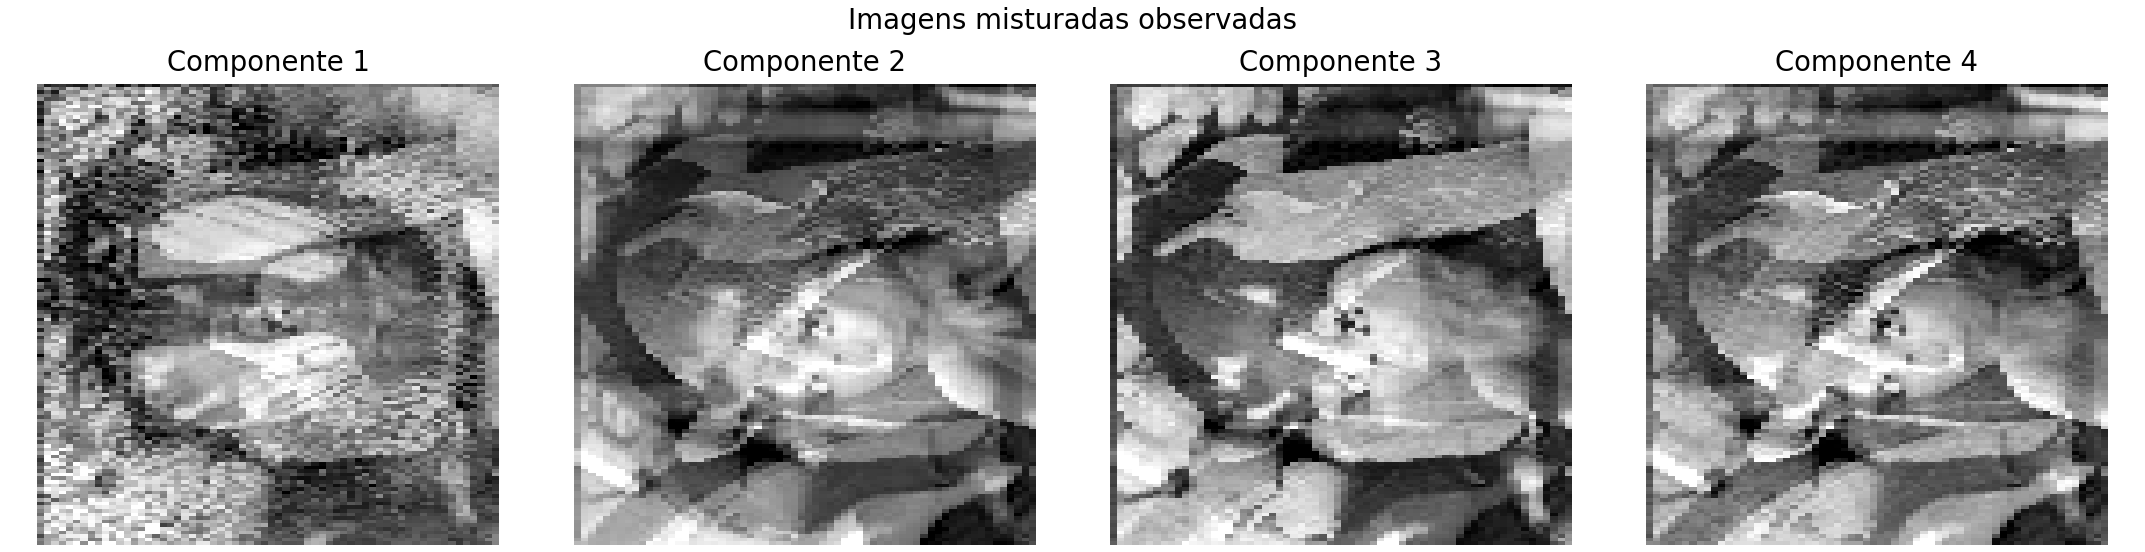
\includegraphics[width=\textwidth]{misturas.png}\caption{Imagens observadas após normalização por percentis apenas para visualização.}\end{figure}
\begin{figure}[H]\centering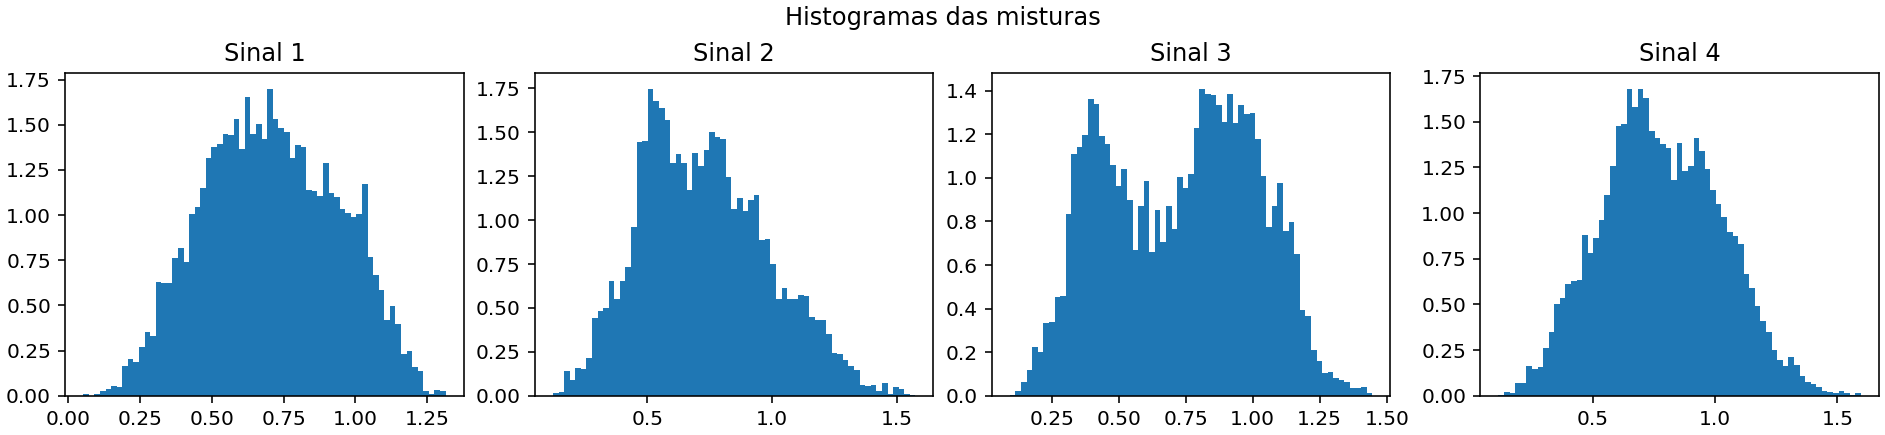
\includegraphics[width=\textwidth]{hist_misturas.png}\caption{Distribuições dos valores observados.}\end{figure}
\begin{figure}[H]\centering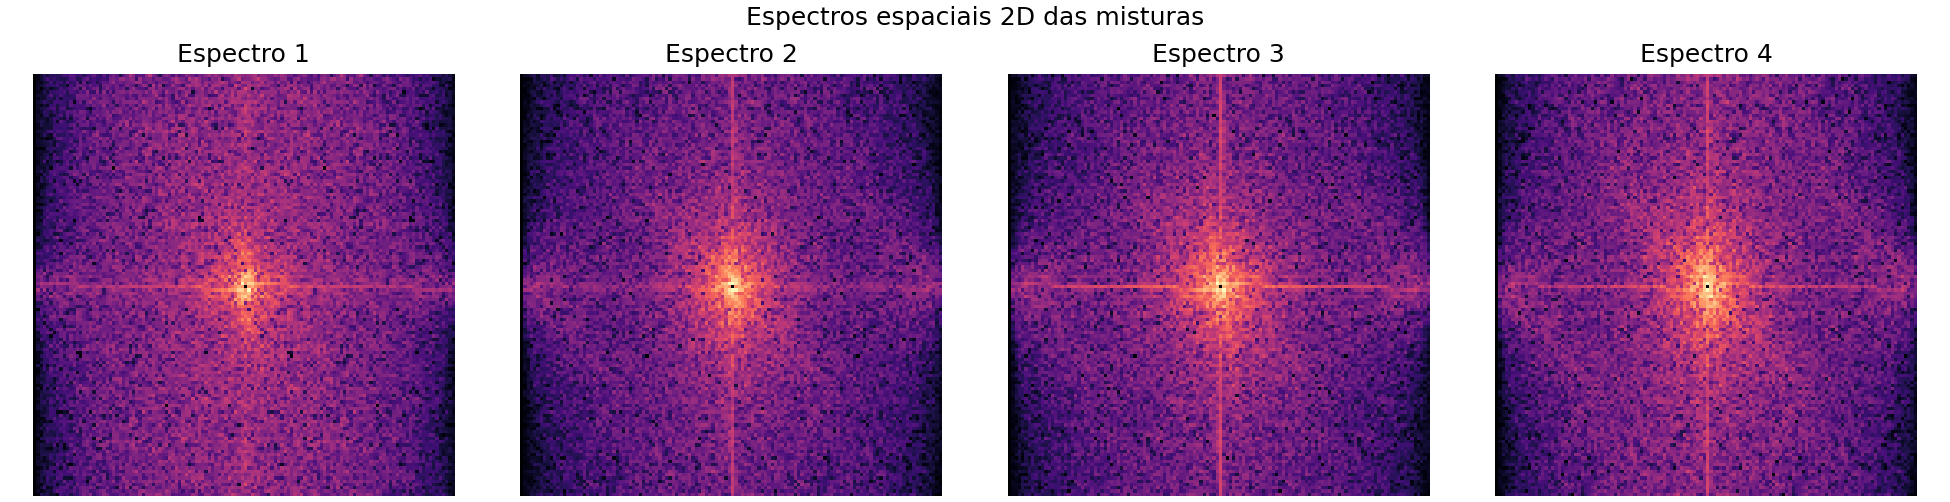
\includegraphics[width=\textwidth]{espectros_misturas.png}\caption{Magnitude logarítmica da FFT espacial 2D centralizada, após remoção da média.}\end{figure}

A alta correlação entre os sinais (correlação absoluta média 0,7282) é coerente com mistura linear. A separação pode ser dificultada por texturas, estruturas espaciais correlacionadas, iluminação e ausência de garantia de independência estatística entre imagens reais.

\section{Modelo matemático e pré-processamento}
Assume-se uma mistura linear instantânea \(X_c=SA^\top\), com amostras nas linhas e canais nas colunas, após a remoção da média \(X_c=X-\boldsymbol{1}\mu^\top\). O ICA estima \(\widehat S=X_cB\), sem conhecer \(S\) ou \(A\). É inerente ao modelo a ambiguidade de permutação, escala e sinal.

O branqueamento diagonaliza \(\Sigma_X=E\Lambda E^\top\) e transforma os dados conforme \(Z=X_cE\Lambda^{-1/2}\), cuja covariância se aproxima da identidade. Os quatro autovalores são mantidos; não se aplica redução dimensional. O FastICA realiza centralização e branqueamento internamente; o experimento JADE utiliza branqueamento explícito.

\section{Algoritmos e parâmetros}
\subsection{FastICA — experimento principal}
O FastICA procura direções que maximizem a não gaussianidade por iteração de ponto fixo. Utilizou-se a implementação \texttt{sklearn.decomposition.FastICA}, com \texttt{n\_components=4}, \texttt{algorithm='parallel'}, \texttt{whiten='unit-variance'}, contraste \texttt{logcosh}, \texttt{tol=1e-6}, \texttt{max\_iter=2000} e semente 42. O algoritmo terminou após 6 iterações. A não gaussianidade é uma condição favorável à identificabilidade da ICA sob hipóteses adequadas, mas não equivale a comprovação de fontes físicas recuperadas.

\subsection{JADE — experimento adicional}
A segunda abordagem constrói matrizes de cumulantes de quarta ordem dos dados branqueados, usando
\begin{equation}
Q^{(ij)}_{ab}=\operatorname{cum}(z_a,z_b,z_i,z_j)
=\mathbb E[z_az_bz_iz_j]-\delta_{ab}\delta_{ij}-\delta_{ai}\delta_{bj}-\delta_{aj}\delta_{bi}.
\end{equation}
A diagonalização conjunta minimiza a energia dos elementos fora da diagonal de \(R^\top Q^{(ij)}R\), sujeita a \(R^\top R=I\). A implementação apresentada parametriza \(R\) por seis rotações planas e otimiza essa função por BFGS com quatro inicializações. Trata-se de uma \textbf{implementação de abordagem JADE por otimização ortogonal}, e não de uma biblioteca JADE de referência com varreduras Jacobi. O otimizador informou \textit{success=false} (possível limitação de precisão numérica); portanto, a solução é tratada como aproximação encontrada, sem alegar convergência certificada para o mínimo global.

\section{Componentes independentes estimadas}
\begin{figure}[H]\centering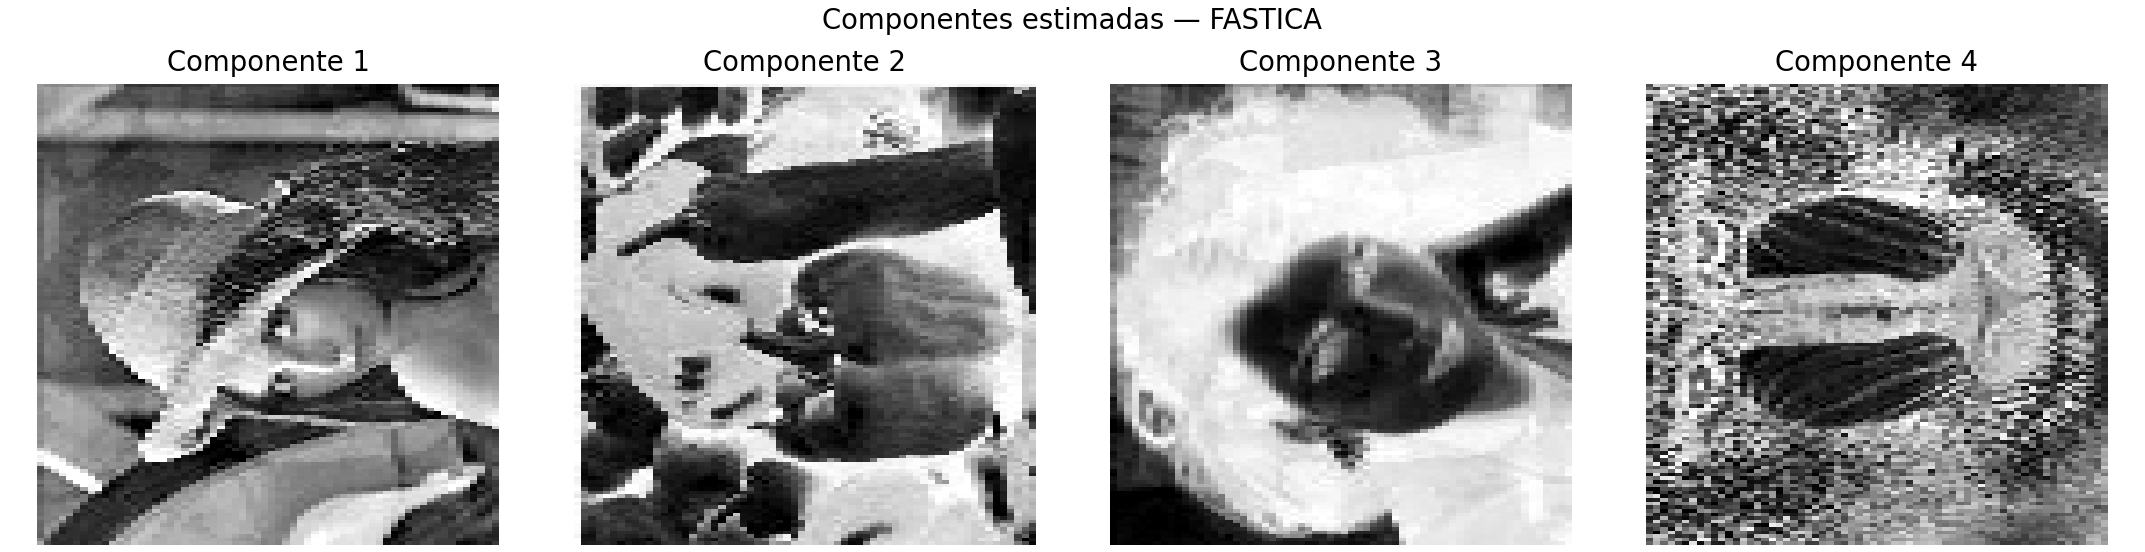
\includegraphics[width=\textwidth]{componentes_fastica.png}\caption{Quatro componentes estimadas pelo FastICA. Contraste e escala são ajustados apenas para exibição.}\end{figure}
\begin{figure}[H]\centering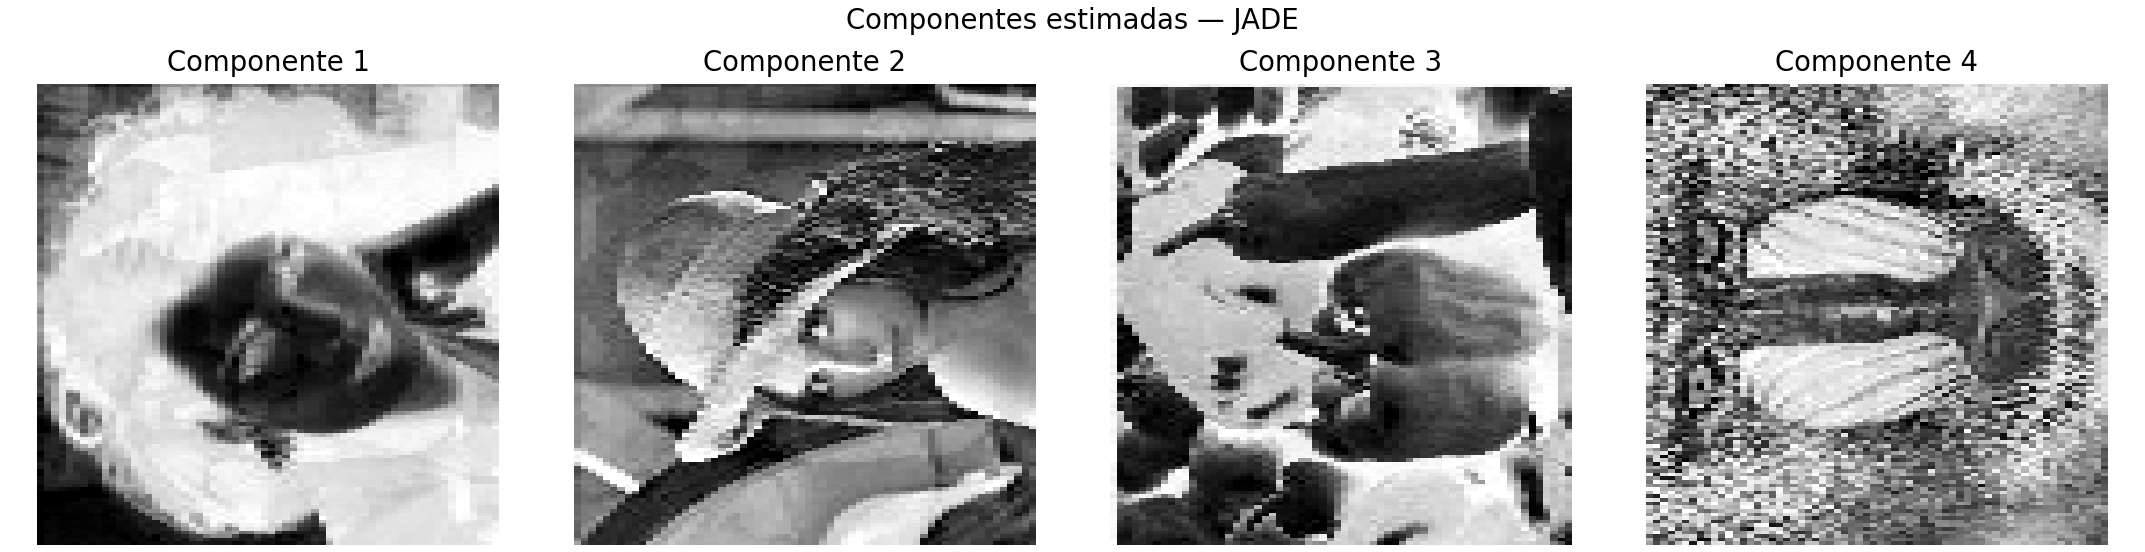
\includegraphics[width=\textwidth]{componentes_jade.png}\caption{Quatro componentes estimadas por diagonalização conjunta de cumulantes.}\end{figure}
\begin{figure}[H]\centering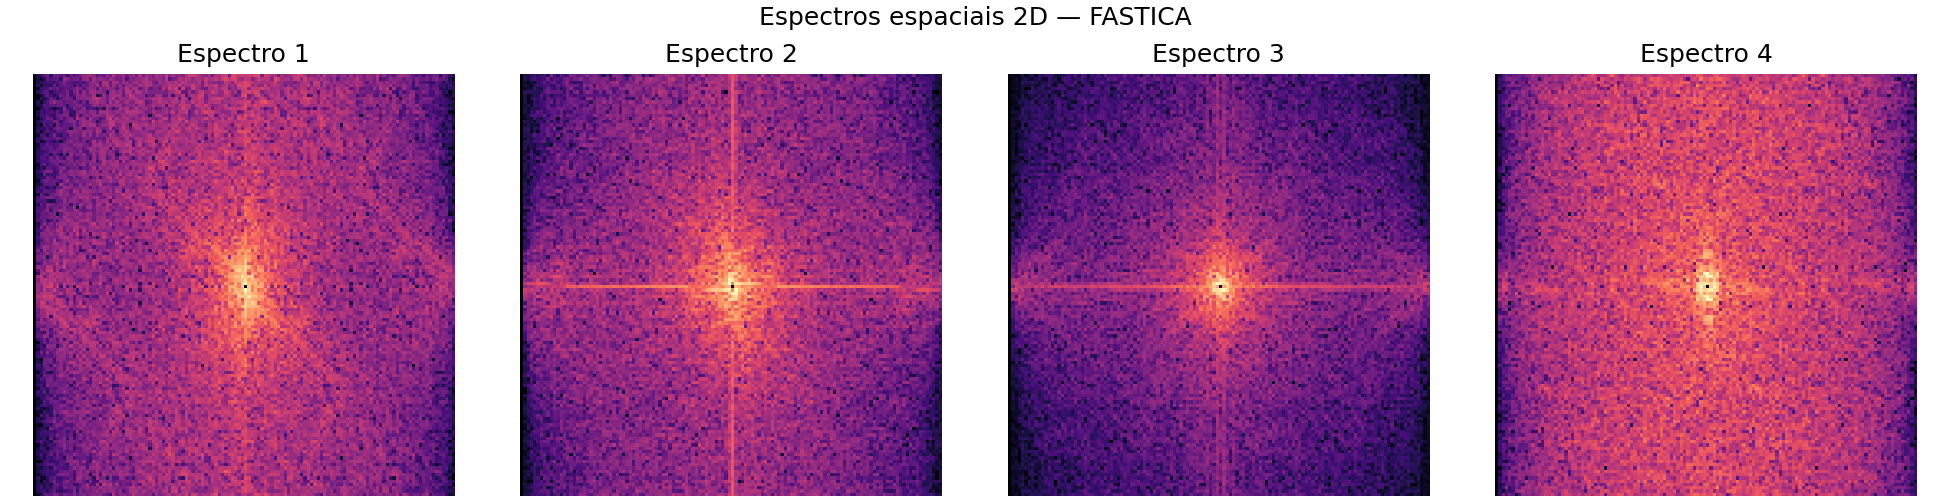
\includegraphics[width=\textwidth]{espectros_fastica.png}\caption{Espectros espaciais das componentes estimadas por FastICA.}\end{figure}
\begin{figure}[H]\centering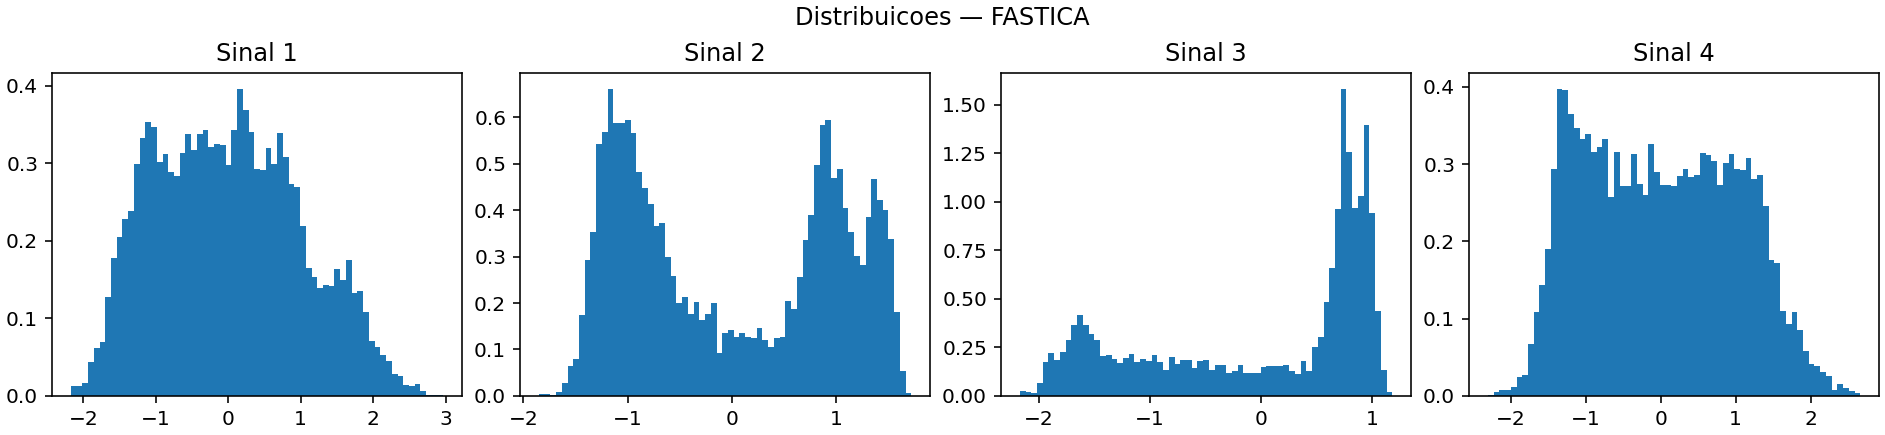
\includegraphics[width=\textwidth]{hist_fastica.png}\caption{Histogramas das componentes FastICA.}\end{figure}

As componentes têm padrões visuais distintos; contudo, exibem também estruturas e texturas que podem refletir vazamento entre fontes. A aparência visual é evidência exploratória, não prova de independência nem identidade com imagens originais.

\section{Avaliação quantitativa da independência}
A correlação absoluta média é calculada sobre os seis pares diferentes de componentes:
\(\overline{|r|}=\frac{2}{k(k-1)}\sum_{i<j}|\mathrm{corr}(s_i,s_j)|\).
A informação mútua (IM) é estimada em \textbf{5.000 pixels amostrados sem reposição}, por regressão de vizinhos mais próximos (\(k=5\)), com média das duas orientações por par. A IM estimada é sensível ao estimador e à amostragem; todos os métodos foram avaliados com o mesmo procedimento. A curtose reportada é o excesso de curtose (normal igual a zero).

\begin{table}[H]\centering
\caption{Comparação quantitativa (resultados da execução com o arquivo disponibilizado).}
\begin{tabular}{lrrr}\toprule
Métrica & Misturas & FastICA & JADE aprox. \\\midrule
Correlação absoluta média & 0,728191 & $4,80\times10^{-15}$ & $8,58\times10^{-16}$ \\
IM média estimada (nats) & 0,680016 & 0,181155 & 0,194420 \\
Erro relativo de reconstrução & 0 & $2,56\times10^{-16}$ & $2,63\times10^{-16}$ \\
\bottomrule\end{tabular}
\end{table}

As componentes FastICA apresentaram excesso de curtose de aproximadamente \(-0,707,-1,571,-1,159,-1,035\). Para a solução JADE, os valores foram \(-1,156,-0,711,-1,579,-1,026\), sujeitos a permutações das componentes. Todos são diferentes de zero, indicando distribuições não gaussianas nesta amostra; não há equivalência direta entre maior curtose absoluta e separação correta. A IM média menor do FastICA sugere menor dependência estimada \textit{nesse critério e amostragem}, mas a diferença é modesta e não estabelece superioridade universal.

\begin{figure}[H]\centering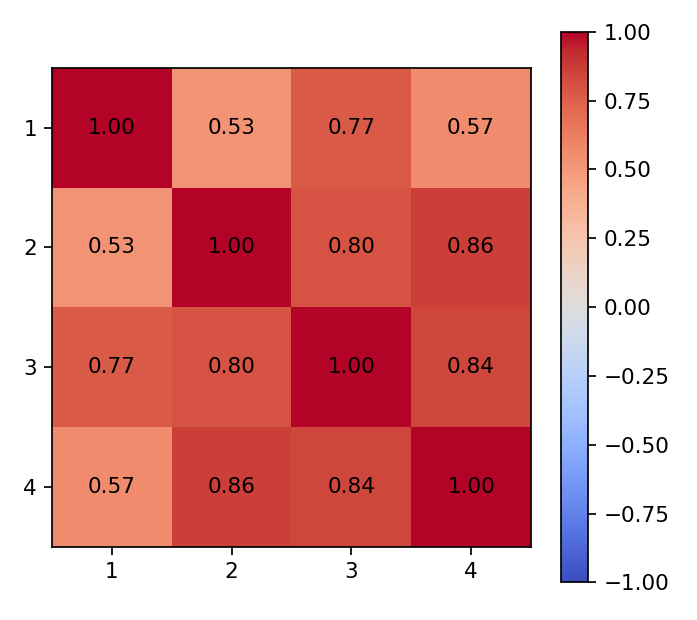
\includegraphics[width=.48\textwidth]{correlacao_misturas.png}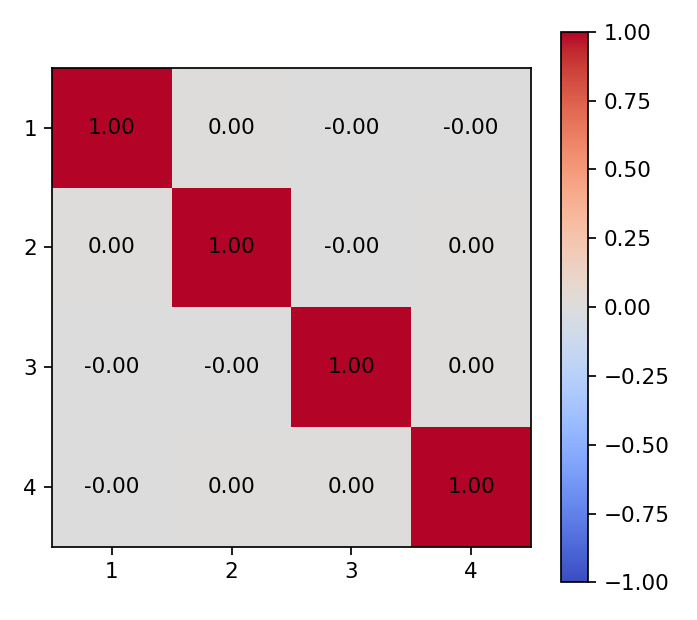
\includegraphics[width=.48\textwidth]{correlacao_fastica.png}\caption{Matrizes de correlação antes (esquerda) e depois do FastICA (direita).}\end{figure}

\section{Reconstrução dos sinais observados}
A reconstrução é obtida pela transformação inversa: \(\widehat X=\widehat S\widehat A^\top+\boldsymbol{1}\mu^\top\). O erro relativo \(\|X-\widehat X\|_F/\|X\|_F\) foi \(2,56\times10^{-16}\) no FastICA e \(2,63\times10^{-16}\) no JADE aproximado. Estes valores próximos da precisão de máquina confirmam consistência algébrica com quatro componentes de posto completo, \textbf{não} uma validação de recuperação das fontes.
\begin{figure}[H]\centering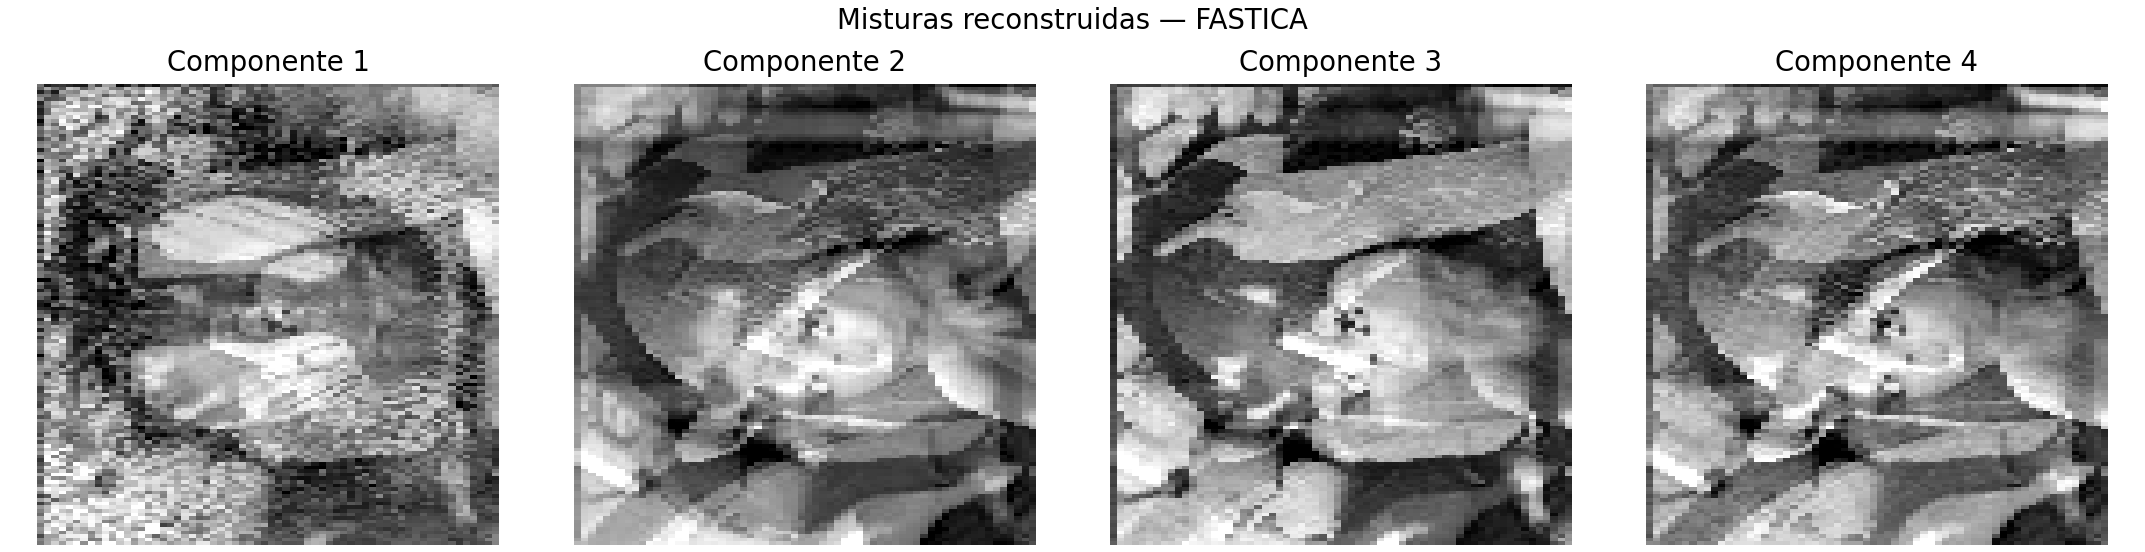
\includegraphics[width=\textwidth]{reconstrucao_fastica.png}\caption{Reconstrução das quatro imagens misturadas a partir das componentes FastICA.}\end{figure}

\section{Discussão crítica e limitações}
\begin{enumerate}
\item \textbf{Há indícios de independência?} Sim: correlação residual praticamente nula e diminuição da informação mútua estimada, embora independência perfeita não tenha sido demonstrada.
\item \textbf{Quais pares permanecem dependentes?} Para o FastICA, o maior par apresenta IM estimada de aproximadamente 0,357 nat (componentes 2 e 3); para a solução JADE aproximada, cerca de 0,443 nat (componentes 1 e 3). A numeração é arbitrária entre execuções e algoritmos.
\item \textbf{As fontes verdadeiras foram recuperadas?} Não é possível afirmar sem \textit{ground truth}; escala, sinal e ordem permanecem indeterminados.
\item \textbf{Quais limitações?} Número reduzido de imagens, hipótese de mistura linear, não independência exata de cenas reais, IM estimada e possível ótimo local ou precisão limitada no método JADE.
\item \textbf{O que permitiria avaliação mais objetiva?} Imagens originais, matriz de mistura ou dados sintéticos controlados, permitindo métricas de separação e comparação por alinhamento/permutações.
\item \textbf{Dificuldades?} Reconstruir a disposição 2D correta a partir de vetores MATLAB; distinguir descorrelação de independência; interpretar ambiguidades de ICA; monitorar a qualidade da diagonalização conjunta.
\end{enumerate}

\section{Reprodutibilidade e conclusões}
Para reprodução: \texttt{pip install -r requirements.txt}; depois \texttt{python experimento.py --input ../mist\_images.mat}. O script gera figuras, \texttt{resultados.json} e arquivos NPZ com as componentes. Recomendam-se Python 3.11+ e o controle de versão de dependências. Os tempos de execução são dependentes do hardware e não devem ser interpretados isoladamente.

Ambas as abordagens produziram componentes descorrelacionadas e reconstrução algébrica fiel. O FastICA apresentou menor informação mútua média estimada nesta execução e não indicou problema de convergência; assim é a solução preferida sob os critérios adotados. A ausência das fontes originais impede qualquer afirmação de separação exata. O experimento confirma que a avaliação em BSS genuinamente cega depende de métricas indiretas, análise visual e discussão cuidadosa das hipóteses.

\begin{thebibliography}{9}
\bibitem{hyvarinen} HYVÄRINEN, A.; KARHUNEN, J.; OJA, E. \textit{Independent Component Analysis}. Wiley, 2001.
\bibitem{cardoso} CARDOSO, J.-F.; SOULOUMIAC, A. Blind beamforming for non-Gaussian signals. \textit{IEE Proceedings F}, v. 140, n. 6, 1993.
\bibitem{sklearn} SCIKIT-LEARN DEVELOPERS. \textit{FastICA Documentation}. \url{https://scikit-learn.org/stable/modules/generated/sklearn.decomposition.FastICA.html}.
\end{thebibliography}
\end{document}
